% GNUPLOT: LaTeX picture with Postscript
\begingroup
  \makeatletter
  \providecommand\color[2][]{%
    \GenericError{(gnuplot) \space\space\space\@spaces}{%
      Package color not loaded in conjunction with
      terminal option `colourtext'%
    }{See the gnuplot documentation for explanation.%
    }{Either use 'blacktext' in gnuplot or load the package
      color.sty in LaTeX.}%
    \renewcommand\color[2][]{}%
  }%
  \providecommand\includegraphics[2][]{%
    \GenericError{(gnuplot) \space\space\space\@spaces}{%
      Package graphicx or graphics not loaded%
    }{See the gnuplot documentation for explanation.%
    }{The gnuplot epslatex terminal needs graphicx.sty or graphics.sty.}%
    \renewcommand\includegraphics[2][]{}%
  }%
  \providecommand\rotatebox[2]{#2}%
  \@ifundefined{ifGPcolor}{%
    \newif\ifGPcolor
    \GPcolorfalse
  }{}%
  \@ifundefined{ifGPblacktext}{%
    \newif\ifGPblacktext
    \GPblacktexttrue
  }{}%
  % define a \g@addto@macro without @ in the name:
  \let\gplgaddtomacro\g@addto@macro
  % define empty templates for all commands taking text:
  \gdef\gplbacktext{}%
  \gdef\gplfronttext{}%
  \makeatother
  \ifGPblacktext
    % no textcolor at all
    \def\colorrgb#1{}%
    \def\colorgray#1{}%
  \else
    % gray or color?
    \ifGPcolor
      \def\colorrgb#1{\color[rgb]{#1}}%
      \def\colorgray#1{\color[gray]{#1}}%
      \expandafter\def\csname LTw\endcsname{\color{white}}%
      \expandafter\def\csname LTb\endcsname{\color{black}}%
      \expandafter\def\csname LTa\endcsname{\color{black}}%
      \expandafter\def\csname LT0\endcsname{\color[rgb]{1,0,0}}%
      \expandafter\def\csname LT1\endcsname{\color[rgb]{0,1,0}}%
      \expandafter\def\csname LT2\endcsname{\color[rgb]{0,0,1}}%
      \expandafter\def\csname LT3\endcsname{\color[rgb]{1,0,1}}%
      \expandafter\def\csname LT4\endcsname{\color[rgb]{0,1,1}}%
      \expandafter\def\csname LT5\endcsname{\color[rgb]{1,1,0}}%
      \expandafter\def\csname LT6\endcsname{\color[rgb]{0,0,0}}%
      \expandafter\def\csname LT7\endcsname{\color[rgb]{1,0.3,0}}%
      \expandafter\def\csname LT8\endcsname{\color[rgb]{0.5,0.5,0.5}}%
    \else
      % gray
      \def\colorrgb#1{\color{black}}%
      \def\colorgray#1{\color[gray]{#1}}%
      \expandafter\def\csname LTw\endcsname{\color{white}}%
      \expandafter\def\csname LTb\endcsname{\color{black}}%
      \expandafter\def\csname LTa\endcsname{\color{black}}%
      \expandafter\def\csname LT0\endcsname{\color{black}}%
      \expandafter\def\csname LT1\endcsname{\color{black}}%
      \expandafter\def\csname LT2\endcsname{\color{black}}%
      \expandafter\def\csname LT3\endcsname{\color{black}}%
      \expandafter\def\csname LT4\endcsname{\color{black}}%
      \expandafter\def\csname LT5\endcsname{\color{black}}%
      \expandafter\def\csname LT6\endcsname{\color{black}}%
      \expandafter\def\csname LT7\endcsname{\color{black}}%
      \expandafter\def\csname LT8\endcsname{\color{black}}%
    \fi
  \fi
    \setlength{\unitlength}{0.0500bp}%
    \ifx\gptboxheight\undefined%
      \newlength{\gptboxheight}%
      \newlength{\gptboxwidth}%
      \newsavebox{\gptboxtext}%
    \fi%
    \setlength{\fboxrule}{0.5pt}%
    \setlength{\fboxsep}{1pt}%
\begin{picture}(7200.00,5040.00)%
    \gplgaddtomacro\gplbacktext{%
      \csname LTb\endcsname%
      \put(1342,704){\makebox(0,0)[r]{\strut{}$0$}}%
      \put(1342,1163){\makebox(0,0)[r]{\strut{}$500000$}}%
      \put(1342,1623){\makebox(0,0)[r]{\strut{}$1\times10^{6}$}}%
      \put(1342,2082){\makebox(0,0)[r]{\strut{}$1.5\times10^{6}$}}%
      \put(1342,2542){\makebox(0,0)[r]{\strut{}$2\times10^{6}$}}%
      \put(1342,3001){\makebox(0,0)[r]{\strut{}$2.5\times10^{6}$}}%
      \put(1342,3460){\makebox(0,0)[r]{\strut{}$3\times10^{6}$}}%
      \put(1342,3920){\makebox(0,0)[r]{\strut{}$3.5\times10^{6}$}}%
      \put(1342,4379){\makebox(0,0)[r]{\strut{}$4\times10^{6}$}}%
      \put(1474,484){\makebox(0,0){\strut{}$0$}}%
      \put(2007,484){\makebox(0,0){\strut{}$200$}}%
      \put(2540,484){\makebox(0,0){\strut{}$400$}}%
      \put(3073,484){\makebox(0,0){\strut{}$600$}}%
      \put(3606,484){\makebox(0,0){\strut{}$800$}}%
      \put(4139,484){\makebox(0,0){\strut{}$1000$}}%
      \put(4671,484){\makebox(0,0){\strut{}$1200$}}%
      \put(5204,484){\makebox(0,0){\strut{}$1400$}}%
      \put(5737,484){\makebox(0,0){\strut{}$1600$}}%
      \put(6270,484){\makebox(0,0){\strut{}$1800$}}%
      \put(6803,484){\makebox(0,0){\strut{}$2000$}}%
      \put(4139,850){\rotatebox{12}{\makebox(0,0)[l]{\strut{}$1/3n^2$}}}%
      \put(3500,1350){\rotatebox{32}{\makebox(0,0)[l]{\strut{}$n^2$}}}%
    }%
    \gplgaddtomacro\gplfronttext{%
      \csname LTb\endcsname%
      \put(176,2541){\rotatebox{-270}{\makebox(0,0){\strut{}Operation Count}}}%
      \put(4138,154){\makebox(0,0){\strut{}Input Size}}%
      \put(4138,4709){\makebox(0,0){\strut{}Empirical Analysis of Brute Force Closest Pair Problem}}%
    }%
    \gplbacktext
    \put(0,0){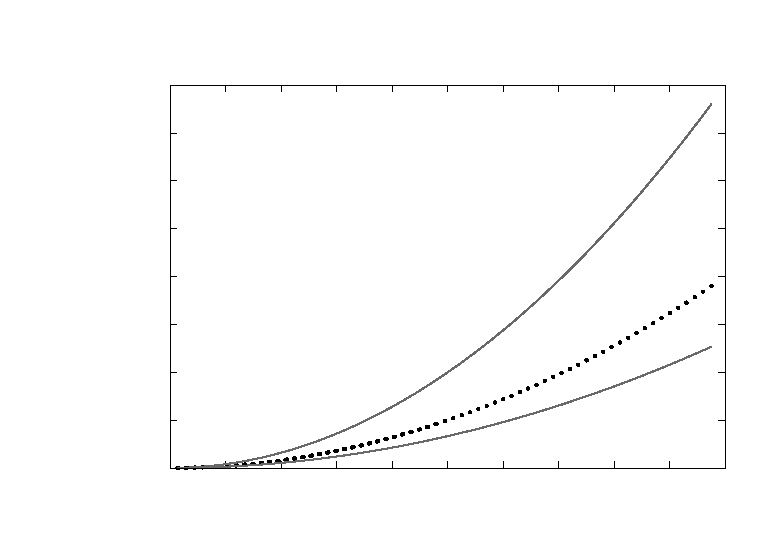
\includegraphics{output_bf}}%
    \gplfronttext
  \end{picture}%
\endgroup
